\documentclass[11pt]{article}

% ---------- Paquetes ----------
\usepackage[spanish]{babel}
\usepackage[utf8]{inputenc}
\usepackage[T1]{fontenc}
\usepackage{amsmath, amssymb}
\usepackage{geometry}
\usepackage[hyphens]{url}
\usepackage{hyperref}
\usepackage{enumitem}
\usepackage{booktabs}
\usepackage{graphicx}
\usepackage{float}
\usepackage{tikz}
\usetikzlibrary{arrows.meta, positioning}

\geometry{margin=2.5cm}
\hypersetup{colorlinks=true, linkcolor=black, urlcolor=blue}
\graphicspath{{figuras/}}

% ---------- Datos del documento ----------
\title{Caracterización del Viento en las Zonas de Operación\\
\large Obtención, organización y uso de los datos para el diseño del UAV}
\author{Ivna}
\date{\today}

\begin{document}
\shorthandoff{<>}

\maketitle

\begin{abstract}
Este documento describe cómo se caracteriza el viento en las dos zonas de
operación previstas para el UAV --el yacimiento Cañadón León (Santa Cruz) y
el área Puesto Hernández (límite Neuquén--Mendoza)-- y cómo esa información se
incorpora al diseño. Se detalla la fuente de los datos (reanálisis ERA5), su
validación contra estaciones meteorológicas reales, la forma en que se
organizan para que el código los consuma independientemente de la geometría
del ala, y sus dos usos: fijar requisitos de misión (velocidad de crucero,
densidad de diseño) y definir las perturbaciones de viento (ráfagas,
gradiente vertical, turbulencia) que se introducen en el análisis VLM y en el
dimensionamiento estructural. Por último, se describe el código que implementa
todo lo anterior y su aplicación a los diseños ganadores del optimizador
multi-topología (misión de crucero a 80~km/h y velocidad máxima de 120~km/h).
\end{abstract}

\tableofcontents

% ======================================================
\section{Introducción: qué parte del viento le importa al ala}
\label{sec:intro}
% ======================================================

\textbf{Intuición:} pensá en caminar dentro de un tren en movimiento. El tren
puede ir a 100~km/h, pero adentro no sentís ningún viento: te movés junto con
el aire del vagón. Con el avión pasa lo mismo. Un viento \emph{uniforme} --el
mismo en todos lados y en todo momento-- desplaza toda la masa de aire, y el
avión vuela ``dentro'' de ella sin notar ninguna diferencia aerodinámica. Lo
único que cambia es su velocidad respecto del suelo: con viento en contra
avanza más lento, con viento a favor más rápido.

Lo que el ala sí ``siente'' son las \textbf{diferencias} de viento: que el
aire se mueva distinto en distintos puntos del espacio o en distintos
instantes. Esto separa naturalmente el problema en dos partes, que conviene
no mezclar:

\begin{description}[leftmargin=3.2cm, style=nextline]
  \item[Viento medio] Afecta la \emph{misión}: alcance, tiempo de vuelo,
  energía, operabilidad. No entra al VLM.
  \item[Variaciones del viento] Afectan la \emph{aerodinámica y la
  estructura}: ráfagas, gradiente vertical y turbulencia modifican el ángulo
  de ataque local y generan cargas. Entran al VLM.
\end{description}

Una consecuencia práctica importante: \textbf{el viento es un dato del lugar,
no del avión}. Puede caracterizarse por completo antes de cerrar la geometría
del ala, y sigue siendo válido aunque la geometría cambie.

% ======================================================
\section{Zonas de operación}
\label{sec:zonas}
% ======================================================

Según el relevamiento con Quintana Energy, la misión tipo es el monitoreo de
pozos ubicados a 60--70~km de la base más próxima. Se tomaron como
referencia dos zonas:

\begin{description}[leftmargin=3.6cm, style=nextline]
  \item[Cañadón León] Yacimiento en el noreste de la provincia de Santa Cruz,
  en la Cuenca del Golfo San Jorge. Punto representativo: $46.56^\circ$S,
  $67.62^\circ$O, junto a Cañadón Seco. En la zona existe además un parque
  eólico (YPF Luz), indicador de viento fuerte y sostenido.
  \item[Puesto Hernández] Área de concesión que abarca Neuquén y Mendoza,
  unos 20~km al noroeste de Rincón de los Sauces. Punto representativo:
  $37.27^\circ$S, $69.08^\circ$O. (En el informe figura como ``PIPH''; queda
  pendiente confirmar la sigla con Quintana.)
\end{description}

Los puntos son representativos de cada zona, no de un pozo en particular.
Como se verifica en la Sección~\ref{sec:sensibilidad}, el viento varía poco
dentro de un radio de $\sim$30~km, por lo que un punto por zona alcanza para
rutas de 60--70~km.

% ======================================================
\section{Obtención de los datos}
\label{sec:obtencion}
% ======================================================

\subsection{Fuente principal: reanálisis ERA5}

\textbf{Intuición:} en medio de la estepa no hay estaciones meteorológicas.
Un \textbf{reanálisis} resuelve ese problema: toma todas las observaciones
disponibles en el mundo (estaciones, satélites, radiosondeos, aviones) y las
combina con un modelo físico de la atmósfera para reconstruir, hora por
hora, el estado del aire en una grilla regular --incluso en lugares donde
nadie midió nada--. Es, en esencia, un ``mapa meteorológico del pasado'' sin
huecos.

Se utilizó ERA5, el reanálisis del Centro Europeo (ECMWF) para el servicio
Copernicus, con resolución horizontal de $0.25^\circ$ ($\approx$28$\times$19~km
a estas latitudes). El acceso se realizó mediante la API histórica de
Open-Meteo (sin necesidad de registro). Para cada zona se descargaron
\textbf{10 años completos (2016--2025), hora por hora}: 87\,672 horas, sin
datos faltantes, con las siguientes variables:

\begin{itemize}[nosep]
  \item velocidad y dirección del viento a 10~m y a 100~m sobre el terreno;
  \item ráfaga máxima a 10~m (máxima ráfaga de 3~s de la hora anterior);
  \item temperatura a 2~m y presión en superficie (para la densidad del aire).
\end{itemize}

\subsection{Del viento a 100~m al viento a altura de vuelo}

La altura máxima típica de operación es 120~m sobre el terreno, pero ERA5
entrega el viento a 10 y 100~m. Como el viento crece con la altura (el
suelo lo frena por rozamiento), se usa la \textbf{ley de potencia}:
\begin{equation}
U(z) = U_{ref}\left(\frac{z}{z_{ref}}\right)^{\alpha}
\label{eq:potencia}
\end{equation}
El exponente $\alpha$ no se supone: se calcula para cada hora a partir de los
dos niveles disponibles,
\begin{equation}
\alpha = \frac{\ln(U_{100}/U_{10})}{\ln 10},
\qquad
U_{120} = U_{100}\cdot 1.2^{\alpha}
\end{equation}
La extrapolación de 100 a 120~m es corta (el viento sube $\sim$3\%), por lo que
el error introducido es menor.

\textbf{Intuición sobre $\alpha$:} de día, el sol calienta el suelo, el aire
se mezcla verticalmente y el viento es casi igual a todas las alturas
($\alpha\approx0.10$). De noche, el aire cerca del suelo se enfría y queda
``estancado'', mientras arriba sigue soplando: el viento cambia mucho con la
altura ($\alpha\approx0.25$). Este segundo caso es el más exigente para
despegues y aterrizajes.

\subsection{Densidad del aire}

A partir de la presión y la temperatura se calcula la densidad horaria con
la ecuación de estado del gas ideal (aire seco; el error por humedad es
menor al 1\%):
\begin{equation}
\rho = \frac{p_{sup}}{R\,T}, \qquad R = 287.05~\mathrm{J/(kg\,K)}
\end{equation}
Para diseño se toma el percentil 5 (aire ``fino'', la condición más
desfavorable para sustentar), corregido por los 120~m de altura
($\times0.986$).

\subsection{Validación contra estaciones reales}
\label{sec:validacion}

Un reanálisis promedia el viento sobre una celda de $\sim$25~km, por lo que
tiende a ``suavizar'' los picos. Para cuantificarlo, se comparó ERA5 con las
observaciones de dos estaciones (NOAA NCEI, reportes horarios SYNOP/METAR,
2021--2025, $\sim$40\,000 horas emparejadas cada una), usando las mismas
horas en ambas series (Tabla~\ref{tab:validacion},
Figura~\ref{fig:validacion}).

\begin{table}[H]
\centering
\small
\begin{tabular}{@{}lcccc@{}}
\toprule
Estación & Media (obs./ERA5) & p90 (obs./ERA5) & p99 (obs./ERA5) & Correlación \\
\midrule
Comodoro Rivadavia Aero & 5.97 / 5.58 & 11.3 / 9.3 & 16.0 / 12.3 & 0.79 \\
Neuquén Aero & 2.61 / 3.75 & 5.7 / 6.9 & 9.3 / 10.1 & 0.75 \\
\bottomrule
\end{tabular}
\caption{Viento a 10~m [m/s] observado vs.\ ERA5 en la celda de cada estación.}
\label{tab:validacion}
\end{table}

\begin{figure}[H]
\centering
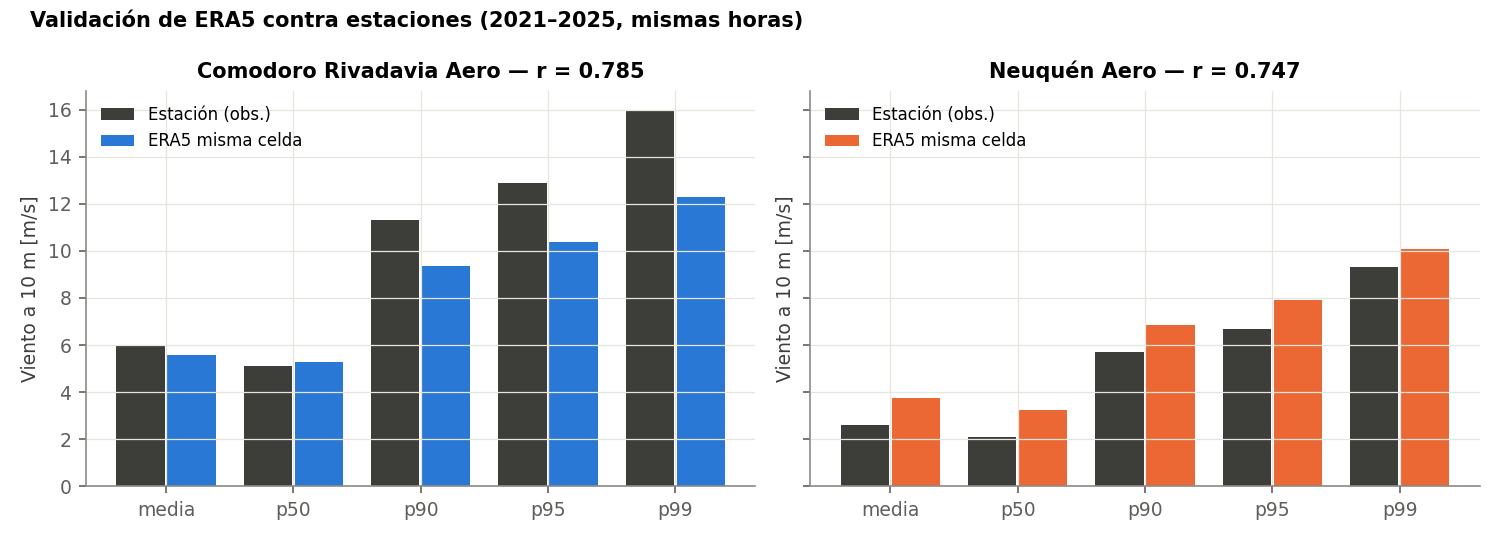
\includegraphics[width=\textwidth]{validacion_era5_estaciones.png}
\caption{Validación de ERA5 contra estaciones (mismas horas, 2021--2025).}
\label{fig:validacion}
\end{figure}

Conclusiones:
\begin{itemize}[nosep]
  \item En la Patagonia (Comodoro Rivadavia), ERA5 acierta en la media pero
  \textbf{subestima los vientos fuertes en un 20--30\%}. Se adopta un
  \textbf{factor de corrección de cola de 1.25} para Cañadón León, aplicado a
  percentiles $\geq$p90 y a valores extremos.
  \item En Neuquén, ERA5 sobreestima la media (la estación está en un valle
  reparado), pero acierta el p99; las ráfagas máximas observadas son
  $\sim$10\% mayores. Se adopta un factor de 1.10 para Puesto Hernández.
  \item Ninguna estación coincide con las zonas de operación, por lo que los
  factores son una estimación razonable, no una corrección exacta. Datos de
  una estación propia del yacimiento (Quintana/YPF) o del parque eólico
  reemplazarían con ventaja a este análisis.
\end{itemize}

\subsection{Sensibilidad espacial}
\label{sec:sensibilidad}

Se evaluaron las cuatro celdas vecinas ($\pm0.25^\circ$) de cada punto. El
viento medio a 100~m varía entre 8.5 y 9.0~m/s en Cañadón León y entre 3.6 y
4.8~m/s en Puesto Hernández: el viento es representativo de la zona, no de un
punto aislado.

\subsection{Turbulencia y ráfagas: normas, no reanálisis}

ERA5 es demasiado ``grueso'' (resolución horaria y de decenas de km) para
representar la turbulencia que siente un ala de un metro. Esta parte se toma
de modelos normalizados y se \emph{escala} con los datos de cada zona:

\begin{description}[leftmargin=3.4cm, style=nextline]
  \item[Turbulencia continua] Modelo de Dryden de baja altura
  ($h<1000$~ft), según MIL-F-8785C y MIL-HDBK-1797.
  \item[Ráfaga discreta] Forma 1$-$coseno, con el factor de alivio de
  ráfaga de FAR/CS-23 (\S23.333 y \S23.341).
\end{description}

El detalle de ambos modelos se desarrolla en la
Sección~\ref{sec:uso-vlm}.

% ======================================================
\section{Organización de los datos}
\label{sec:organizacion}
% ======================================================

\textbf{Intuición:} la organización responde a una regla simple: \emph{cada
número tiene que poder rastrearse hasta su fuente}, y el código no tiene que
saber nada de cómo se obtuvo. Por eso se separa en tres niveles: lo crudo
(que nunca se toca), lo procesado (lo que lee el código) y lo documentado
(lo que lee el tribunal).

Todo se encuentra en la carpeta \texttt{Proyecto final/Datos de viento/}:

\begin{table}[H]
\centering
\begin{tabular}{@{}p{3.6cm}p{6.2cm}p{4.2cm}@{}}
\toprule
Nivel & Contenido & Destinatario \\
\midrule
\texttt{datos/}, \texttt{datos\_crudos/} & Resúmenes estadísticos completos, validación, sensibilidad espacial; serie horaria (se regenera con un script) & Reproducibilidad \\
\texttt{fichas/*.yaml} & Una ficha por zona con los parámetros procesados, con nombre y unidad & Código (VLM, misión, estructura) \\
\texttt{tablas/}, \texttt{figuras/}, \texttt{LEEME} & Tablas CSV, gráficos, supuestos y fuentes & Tesis \\
\texttt{scripts/} & \texttt{descargar\_era5.py}, \texttt{procesar\_viento.py} & Regenerar todo \\
\bottomrule
\end{tabular}
\caption{Estructura de la carpeta de datos de viento.}
\label{tab:carpeta}
\end{table}

Cada ficha contiene, para su zona: ubicación y fuente; densidad del aire;
estadística del viento a 120~m (todas las horas y solo horas diurnas);
viento y ráfagas a 10~m; exponente $\alpha$ del gradiente vertical;
parámetros de turbulencia de Dryden a 120 y 30~m; amplitudes y longitudes de
ráfaga discreta; y extremos para el UAV en tierra.

Agregar una zona nueva no requiere modificar el código de análisis:
basta con generar una ficha nueva. Del mismo modo, cambiar la geometría del
ala no requiere tocar las fichas.

% ======================================================
\section{Resultados}
\label{sec:resultados}
% ======================================================

\begin{table}[H]
\centering
\begin{tabular}{@{}p{5.2cm}cc@{}}
\toprule
A 120~m sobre el terreno & Cañadón León & Puesto Hernández \\
\midrule
Viento medio & 9.2~m/s & 4.3~m/s \\
p90 / p95 / p99 & 14.6 / 16.1 / 19.1~m/s & 8.7 / 10.5 / 13.6~m/s \\
p95 diurno (08--19~h) & 16.3~m/s & 10.9~m/s \\
Dirección dominante & O--ONO ($\approx$40\%) & ENE--E (22\%), SO--O (27\%) \\
Ráfaga a 10~m: p99 / máxima & 22.1 / 36.0~m/s & 17.3 / 28.7~m/s \\
$\alpha$ mediana (día / noche) & 0.18 (0.11 / 0.22) & 0.13 (0.10 / 0.25) \\
Densidad media / de diseño & 1.21 / 1.14~kg/m$^3$ & 1.13 / 1.06~kg/m$^3$ \\
Turbulencia del sitio (Dryden) & moderada & entre ligera y moderada \\
\bottomrule
\end{tabular}
\caption{Resumen de la caracterización del viento (ERA5, 2016--2025, sin
corrección de cola).}
\label{tab:resultados}
\end{table}

Las dos zonas son muy distintas. Cañadón León está dominada por el viento
patagónico del oeste: fuerte, persistente y parejo a lo largo del año y del
día. Puesto Hernández es mucho más calma, con un ciclo diario marcado (mínimo
a la mañana, máximo hacia las 20~h) y mayor viento entre septiembre y enero;
además, al estar a $\sim$670~m de altura, su aire es $\sim$6\% menos denso
(Figuras~\ref{fig:cl} y \ref{fig:ph}).

\begin{figure}[H]
\centering
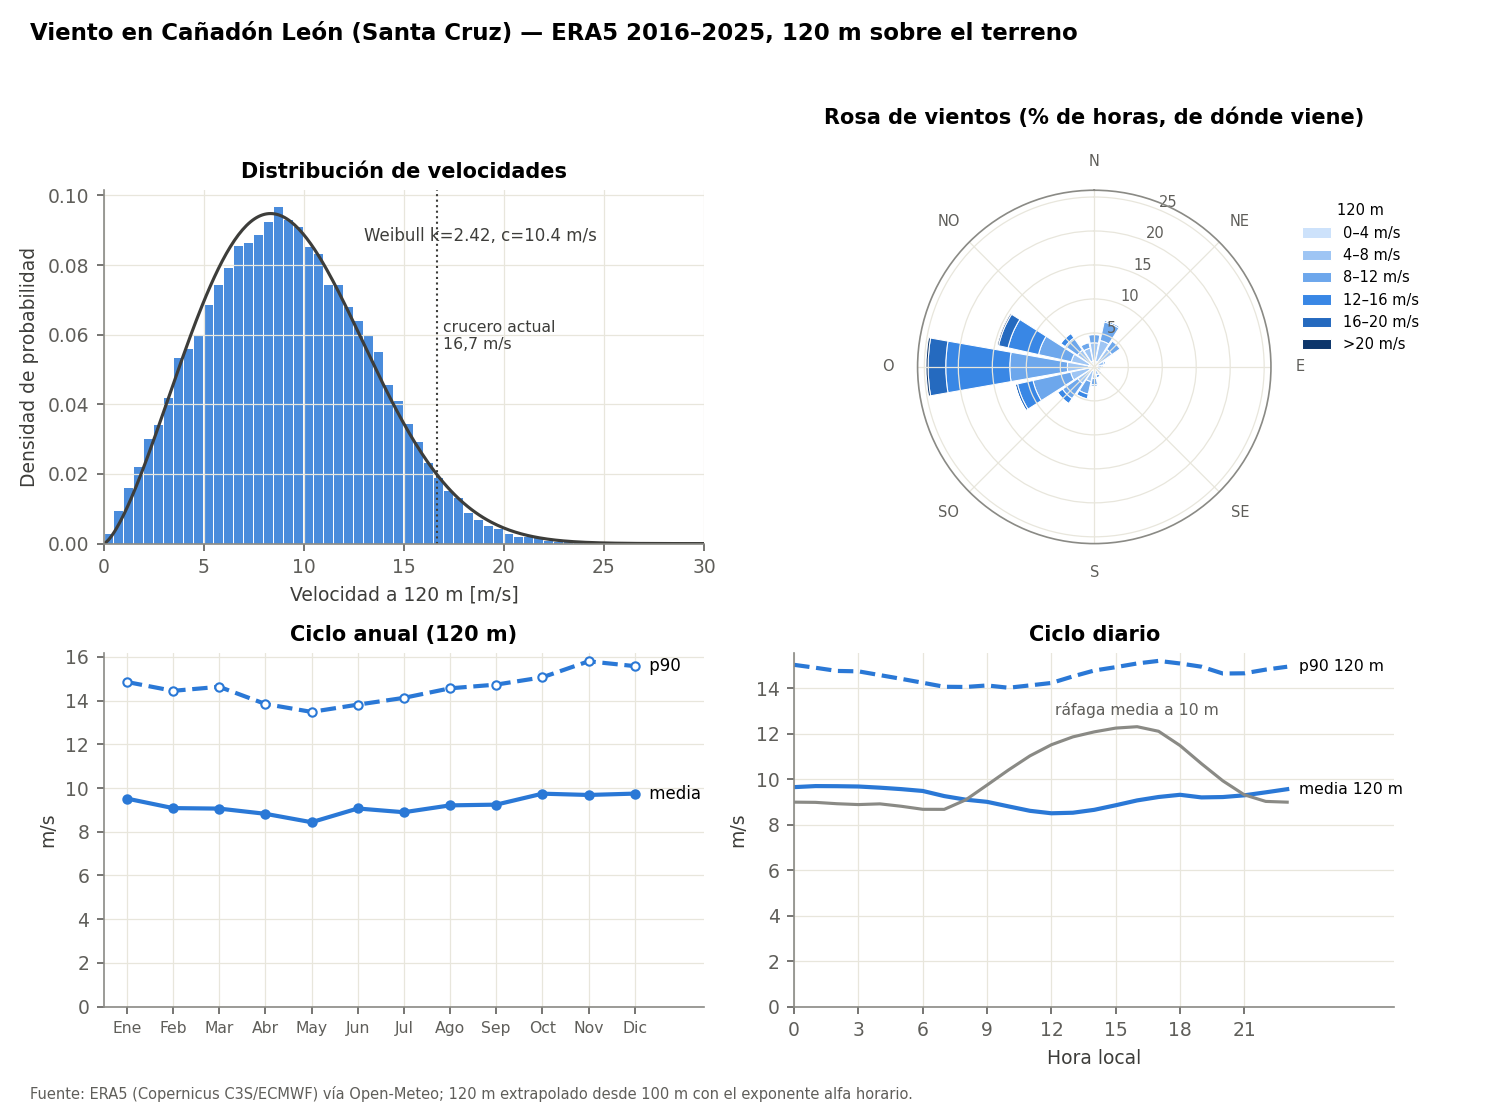
\includegraphics[width=\textwidth]{canadon_leon_panel.png}
\caption{Cañadón León: distribución de velocidades, rosa de vientos, ciclo
anual y ciclo diario a 120~m.}
\label{fig:cl}
\end{figure}

\begin{figure}[H]
\centering
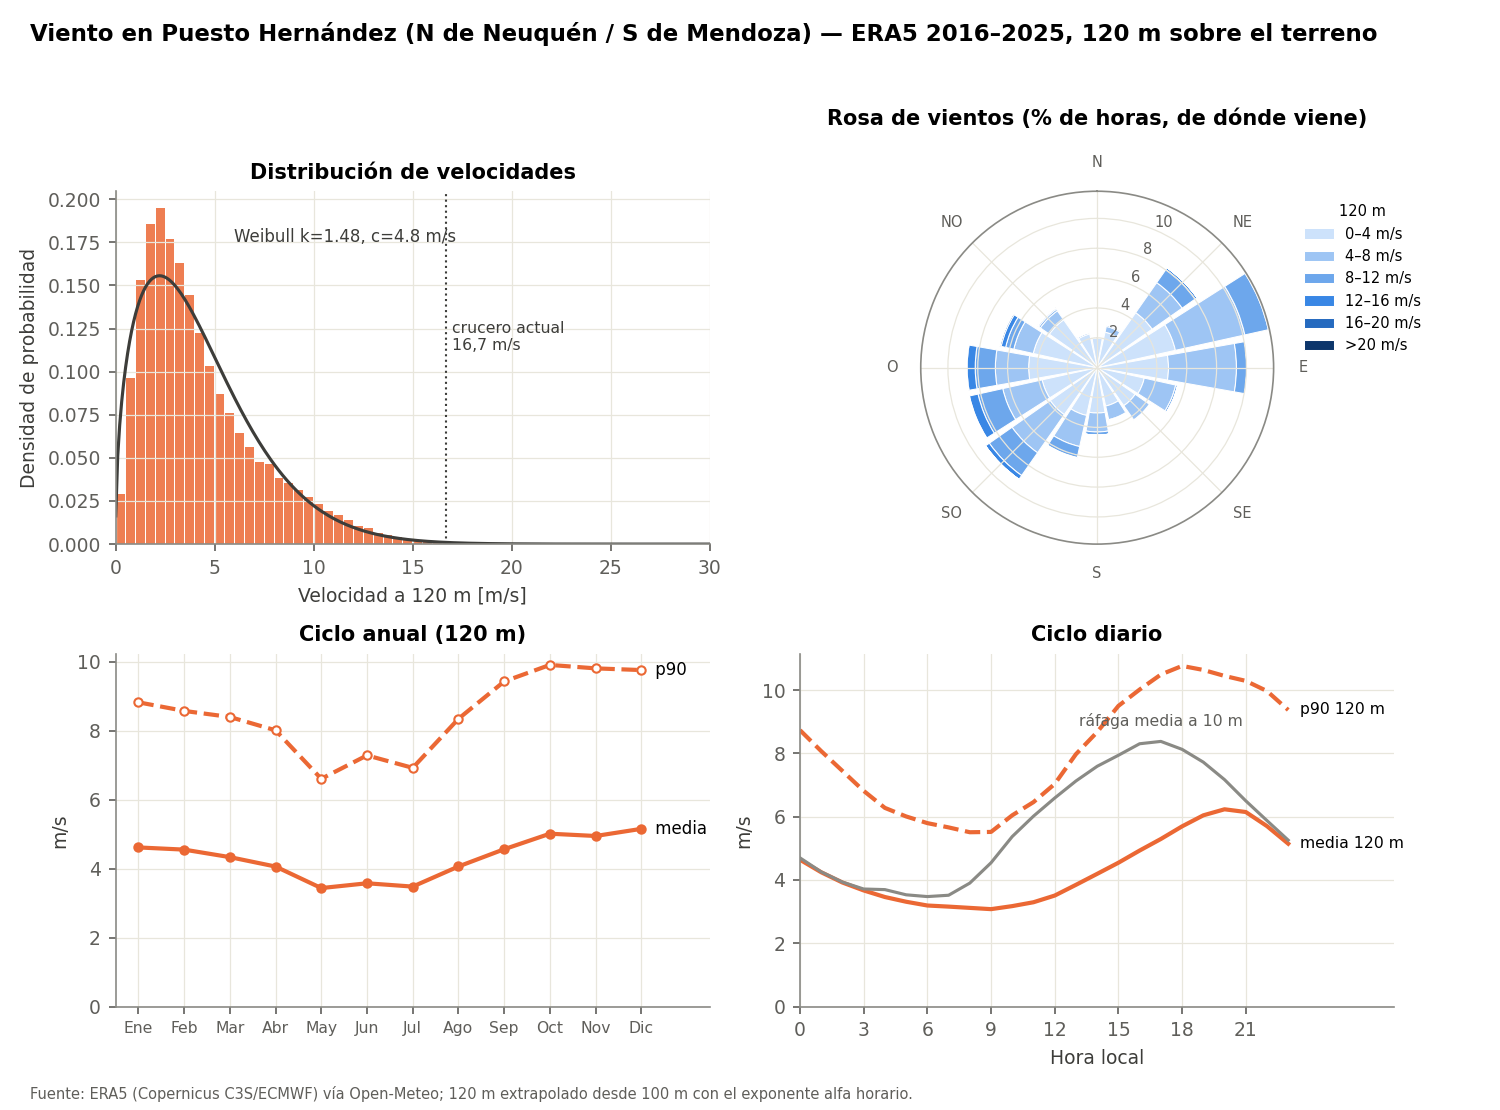
\includegraphics[width=\textwidth]{puesto_hernandez_panel.png}
\caption{Puesto Hernández: distribución de velocidades, rosa de vientos,
ciclo anual y ciclo diario a 120~m.}
\label{fig:ph}
\end{figure}

% ======================================================
\section{Uso de los datos (A): requisitos de misión}
\label{sec:uso-mision}
% ======================================================

\subsection{Velocidad de crucero y operabilidad}

\textbf{Intuición:} un viento en contra no ``cuesta'' lo mismo que lo que
regala un viento a favor. Si volás a 80~km/h con 50~km/h en contra, avanzás
a 30~km/h y tardás 2.7 veces más; a la vuelta, con 50~km/h a favor, avanzás a
130~km/h, pero eso no compensa el tiempo perdido a la ida. Por eso el viento
siempre alarga un viaje de ida y vuelta, y el efecto crece muy rápido cuando
el viento se acerca a la velocidad del avión.

Para un viento $W$ alineado con la ruta (peor caso) y velocidad de crucero
$V_c$, el tiempo de ida y vuelta relativo al de aire quieto es:
\begin{equation}
\frac{t}{t_0} = \frac{1}{1-(W/V_c)^2}
\label{eq:ida-vuelta}
\end{equation}
Se define como \emph{operable} una hora en la que $t/t_0\leq1.5$, es decir,
$W\leq0.577\,V_c$. La Tabla~\ref{tab:operabilidad} muestra el porcentaje de
horas diurnas operables según $V_c$.

\begin{table}[H]
\centering
\small
\begin{tabular}{@{}lccc@{}}
\toprule
Crucero & Cañadón León & C. León (corr. de cola) & Puesto Hernández \\
\midrule
60~km/h (16.7~m/s) & 58\% & 40\% & 92\% \\
72~km/h (20~m/s) & 74\% & 54\% & 96\% \\
\textbf{80~km/h (22.2~m/s), crucero} & \textbf{80\%} & \textbf{63\%} & \textbf{97\%} \\
90~km/h (25~m/s) & 88\% & 74\% & 99\% \\
120~km/h (33.3~m/s), $V_{max}$ & 99\% & 92\% & 100\% \\
\bottomrule
\end{tabular}
\caption{Porcentaje de horas diurnas en que el viaje de ida y vuelta tarda
como máximo 1.5 veces lo que tardaría sin viento.}
\label{tab:operabilidad}
\end{table}

\begin{figure}[H]
\centering
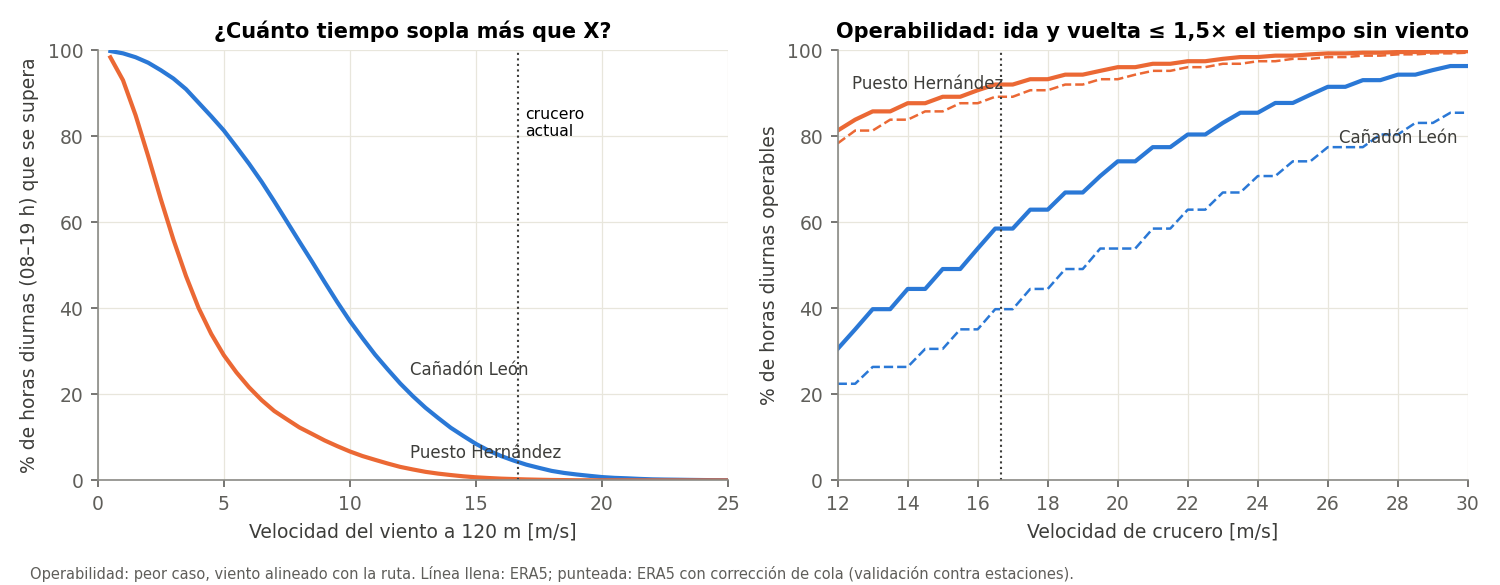
\includegraphics[width=\textwidth]{comparacion_sitios_operabilidad.png}
\caption{Izquierda: fracción de horas diurnas en que se supera cada
velocidad de viento. Derecha: operabilidad en función de la velocidad de
crucero.}
\label{fig:operabilidad}
\end{figure}

\textbf{Consecuencia de diseño:} con la primera misión (crucero a 60~km/h),
en Cañadón León el UAV directamente \emph{no podía avanzar} contra el viento
entre el 5\% y el 17\% de las horas diurnas. La misión actual del
optimizador (crucero de diseño a 80~km/h y velocidad máxima de 120~km/h,
fijada el 18/09/2026 por un análisis de alcance con batería) mejora mucho la
situación: a 80~km/h queda operable el 63--80\% de las horas diurnas en
Cañadón León (sin avance solo el 1--3\%), y la reserva de 120~km/h permite
volver aun con los vientos más fuertes (92--99\%). En Puesto Hernández, la
operabilidad es prácticamente total. Es decir, el requisito de velocidad
máxima que se había fijado ``frente a viento y ráfagas'' queda respaldado
ahora con datos del sitio.

\subsection{Densidad de diseño}

El $C_L$ de crucero necesario es $C_L = W/(\tfrac12\rho V^2 S)$: con aire
menos denso, el ala debe trabajar a mayor $C_L$. Se adopta la densidad de
diseño de la ficha (1.14~kg/m$^3$ en Cañadón León, 1.06~kg/m$^3$ en Puesto
Hernández) en lugar de la densidad estándar a nivel del mar (1.225~kg/m$^3$)
que usa hoy el optimizador. Para los ganadores actuales esto implica un $C_L$
de crucero entre 7\% (Cañadón León) y 16\% (Puesto Hernández) mayor que el
calculado, lo que reduce en esa medida el margen hasta la pérdida.

% ======================================================
\section{Uso de los datos (B): perturbaciones en el VLM y la estructura}
\label{sec:uso-vlm}
% ======================================================

\subsection{Cómo entra el viento en el VLM}

En el VLM se impone, en el punto de control de cada panel $i$, que el flujo
no atraviese la superficie. El viento se incorpora sumando su velocidad
local a la de la corriente libre:
\begin{equation}
\sum_j A_{ij}\,\Gamma_j = -\left(\vec V_\infty + \vec V_{viento}(x_i,y_i,z_i,t)\right)\cdot\hat n_i
\label{eq:vlm-viento}
\end{equation}

\textbf{Intuición:} la matriz $A_{ij}$ solo depende de la geometría del ala,
así que no se toca. Lo único que cambia es el lado derecho: cada panel
``ve'' su propio viento. Por eso el modelo de viento es una función
independiente $\vec V_{viento}(x,y,z,t)$ que recibe coordenadas y devuelve
velocidades, sin saber nada del ala: cambiar la geometría no afecta al
viento, y cambiar de zona no afecta al solver.

Resuelta así en cada instante, la formulación es \textbf{cuasi-estacionaria}:
supone que el ala se adapta instantáneamente a cada nuevo flujo y que el
avión no se mueve por efecto de la ráfaga. Da una cota superior de la carga.
En la Sección~\ref{sec:codigo} se agrega la respuesta dinámica (el avión sube
con la ráfaga y la sustentación tarda en crecer), que es la que se usa para
diseño.

\subsection{Ráfaga discreta 1$-$coseno}

\textbf{Intuición:} es un ``golpe'' de aire vertical que sube suavemente,
llega a un máximo y vuelve a cero. Al sumarse a la velocidad de vuelo, inclina
el viento relativo y le aumenta de golpe el ángulo de ataque al ala,
generando un pico de sustentación (y de carga sobre el larguero).

\begin{equation}
w(x) = \frac{U_{ds}}{2}\left(1-\cos\frac{\pi x}{H}\right),\qquad 0\leq x\leq 2H
\end{equation}
donde $x$ es la distancia recorrida dentro de la ráfaga y $H$ la distancia
hasta el máximo. El incremento de ángulo de ataque efectivo es:
\begin{equation}
\Delta\alpha \approx \arctan\frac{K_g\,U_{ds}}{V},\qquad
K_g = \frac{0.88\,\mu}{5.3+\mu},\qquad
\mu = \frac{2\,(W/S)}{\rho\,\bar c\,C_{L_\alpha}\,g}
\end{equation}
El factor $K_g$ (alivio de ráfaga, FAR~23.341) representa que el avión no
siente la ráfaga entera de golpe: tarda en penetrarla y empieza a responder
mientras tanto.

\textbf{Amplitud de diseño.} La ráfaga de CS-23/FAR~23 (15.24~m/s a $V_C$)
está pensada para aviones tripulados rápidos; en un UAV de $\sim$22~m/s
implicaría $\Delta\alpha\approx19^\circ$, es decir, entrada en pérdida segura.
Se propone en cambio escalar la amplitud con la turbulencia del sitio
(Sección~\ref{sec:dryden}):

\begin{table}[H]
\centering
\small
\begin{tabular}{@{}lcc@{}}
\toprule
Criterio & $U_{ds}$ & $\Delta\alpha$ ($K_g\approx0.50$, $V=22.2$~m/s) \\
\midrule
Operación / suavidad ($2\sigma_w$, turb.\ moderada) & 3.1~m/s & $4.0^\circ$ \\
\textbf{Diseño: margen de pérdida y cargas} ($3\sigma_w$, moderada) & \textbf{4.6~m/s} & $\mathbf{6.0^\circ}$ \\
Nominal Puesto Hernández ($3\sigma_w$, turb.\ ligera) & 2.3~m/s & $3.0^\circ$ \\
Referencia CS-23 a $V_C$ & 15.24~m/s & $\approx19^\circ$ (pérdida) \\
\bottomrule
\end{tabular}
\caption{Amplitudes de ráfaga discreta. El criterio $3\sigma_w$ es una
propuesta propia y debe justificarse como tal.}
\label{tab:rafaga}
\end{table}

La ráfaga de 3~m/s que usa hoy el optimizador (\texttt{mision\_avion.py})
coincide con el criterio de operación ($2\sigma_w$): es adecuada para
puntuar la suavidad de vuelo, pero queda corta como ráfaga de diseño en
Cañadón León. Como $\Delta\alpha\propto U_{ds}/V$, el paso del crucero de
60 a 80~km/h ya redujo este efecto: los $\Delta\alpha$ de la tabla son
$\sim$35\% menores que con la misión original.

\textbf{Longitud de la ráfaga.} CS-23 usa $H=12.5\,\bar c$ (longitud total de
25 cuerdas). Como la carga máxima depende de la relación entre $H$ y la
cuerda, conviene barrer $H$ entre $12.5\,\bar c$ y la escala de turbulencia
vertical a 120~m ($L_w\approx120$~m).

\textbf{Implicancia estructural.} La carga por ráfaga nunca puede superar
la que el ala es capaz de generar antes de entrar en pérdida:
$n\leq C_{L,max}/C_{L,crucero}$. En los ganadores actuales ese tope está
entre 4.3 y 5.4, por encima de la carga de ráfaga de diseño, así que es la
ráfaga (y no la pérdida) la que fija la carga del larguero
(Sección~\ref{sec:codigo}).

\subsection{Gradiente vertical}

En despegue y aterrizaje el ala atraviesa capas de aire con distinta
velocidad. Se modela con la ley de potencia (Ecuación~\ref{eq:potencia}) y el
$\alpha$ de la ficha: $\approx0.10$ de día (cuando se vuela normalmente) y
$\approx0.25$ como caso exigente de aire estable.

\subsection{Turbulencia continua: modelo de Dryden}
\label{sec:dryden}

\textbf{Intuición:} la turbulencia es una sucesión de pequeñas ráfagas
aleatorias sin fin. El modelo de Dryden no intenta predecir cada una, sino
describir su ``carácter'': qué tan fuertes son en promedio ($\sigma$) y qué
tan grandes son los remolinos ($L$). Con eso se generan series aleatorias
realistas para simular el vuelo.

Para baja altura ($h<1000$~ft, con $h$ en pies):
\begin{equation}
\sigma_w = 0.1\,W_{20},\qquad
\frac{\sigma_u}{\sigma_w}=\frac{\sigma_v}{\sigma_w}=\frac{1}{(0.177+0.000823\,h)^{0.4}}
\end{equation}
\begin{equation}
L_w = h,\qquad L_u = L_v = \frac{h}{(0.177+0.000823\,h)^{1.2}}
\quad\text{(MIL-F-8785C)}
\end{equation}
donde $W_{20}$ es el viento a 20~ft (6~m): 15, 30 y 45~kt para turbulencia
ligera, moderada y severa.

Para cada zona se estimó $W_{20}$ a partir del p99 del viento a 10~m
(corregido por el factor de cola). Cañadón León resulta en $W_{20}\approx29$~kt
(moderada) y Puesto Hernández en $\approx19$~kt (entre ligera y moderada). Un
chequeo independiente por teoría de capa límite
($u_*=0.4\,U_{10}/\ln(10/z_0)$, $\sigma_w\approx1.25\,u_*$, $z_0=0.03$~m para
estepa) da $\sigma_w=1.42$~m/s en Cañadón León, coherente con los
1.54~m/s de turbulencia moderada.

\textbf{Se adopta turbulencia moderada como envolvente única de diseño}:
$\sigma_w=1.54$~m/s, $\sigma_u=\sigma_v=2.04$~m/s, $L_w=120$~m y
$L_u=L_v=275$~m a 120~m de altura.

\subsection{Síntesis: qué dato va a dónde}

\begin{figure}[H]
\centering
\begin{tikzpicture}[
  box/.style={draw, rounded corners, align=center, minimum height=1.0cm, text width=3.4cm, font=\small},
  arr/.style={-{Stealth}, thick}]
\node[box] (era) {ERA5 + validación\\(viento por zona)};
\node[box, below=0.9cm of era] (norm) {Normas\\(Dryden, CS-23)};
\node[box, right=1.4cm of era, yshift=-0.95cm] (ficha) {Fichas YAML\\por zona};
\node[box, right=1.4cm of ficha, yshift=0.95cm] (mision) {\textbf{Misión}\\$V_c$, $\rho$, operabilidad};
\node[box, right=1.4cm of ficha, yshift=-0.95cm] (vlm) {\textbf{VLM y estructura}\\ráfaga, gradiente, turbulencia};
\draw[arr] (era) -- (ficha);
\draw[arr] (norm) -- (ficha);
\draw[arr] (ficha) -- node[above, sloped, font=\scriptsize] {viento medio} (mision);
\draw[arr] (ficha) -- node[below, sloped, font=\scriptsize] {variaciones} (vlm);
\end{tikzpicture}
\caption{Flujo de la información de viento desde las fuentes hasta su uso.}
\label{fig:flujo}
\end{figure}

% ======================================================
\section{Implementación en código}
\label{sec:codigo}
% ======================================================

\textbf{Intuición:} todo lo anterior se convierte en un paquete de Python,
\texttt{viento\_uav}, que funciona ``al costado'' del optimizador: no modifica
ninguna línea de ese código. Lee las fichas de cada sitio y, para evaluar un
diseño, solamente usa lo que el optimizador ya produce (el archivo
\texttt{ganadores.json} y la función que arma la geometría).

\subsection{Organización}

\begin{table}[H]
\centering
\small
\begin{tabular}{@{}p{3.4cm}p{10.4cm}@{}}
\toprule
Módulo & Qué hace \\
\midrule
\texttt{fichas.py} & Lee las fichas YAML y el resumen estadístico (histogramas, rosa de vientos). \\
\texttt{campos.py} & Campos de viento componibles: ráfaga 1$-$coseno, ráfaga uniforme, cortante vertical y turbulencia de Dryden sintetizada. \\
\texttt{vlm\_viento.py} & VLM de AeroSandbox con viento no uniforme, paso del avión por un campo (cuasi-estático) y respuesta dinámica a ráfagas. \\
\texttt{mision\_viento.py} & Velocidad respecto del suelo, factor de ida y vuelta, operabilidad con la estadística del sitio y chequeo rápido de ráfaga (FAR~23.341). \\
\texttt{evaluar\_ganadores\_}\newline\texttt{con\_viento.py} & Ejemplo: evalúa los cinco ganadores del optimizador en los dos sitios. \\
\bottomrule
\end{tabular}
\caption{Módulos del paquete \texttt{viento\_uav} (carpeta \texttt{Datos de viento/codigo\_viento}).}
\end{table}

\subsection{Viento en el VLM}

El VLM de AeroSandbox calcula la velocidad del aire en cada panel como la
corriente libre más la velocidad debida a la rotación del avión. El paquete
reemplaza el punto de operación por uno que, en ese mismo cálculo, suma la
velocidad del campo de viento evaluada en cada punto. Así el viento entra
tanto en la condición de no penetración (Ecuación~\ref{eq:vlm-viento}) como
en el cálculo de fuerzas por Kutta--Joukowski, sin tocar la matriz de
influencia.

\subsection{Respuesta dinámica a la ráfaga}

\textbf{Intuición:} en el análisis cuasi-estático el avión queda ``clavado''
mientras la ráfaga lo atraviesa. En la realidad pasan dos cosas que reducen
la carga: el avión empieza a subir empujado por la ráfaga (y entonces la ve
más chica), y la sustentación no aparece de golpe sino que tarda unas
cuerdas de recorrido en desarrollarse. El factor $K_g$ de FAR~23.341 resume
justamente esos dos efectos para un perfil 2D.

Como el VLM es lineal en la velocidad que ve cada panel, la respuesta se
arma en tres pasos:
\begin{enumerate}[nosep]
  \item Con el VLM se calcula la sustentación cuasi-estática $\Delta L_g(X)$
  que produce la ráfaga para cada posición del avión dentro de ella. Esto
  incluye cuándo entra el ala y cuándo entra la cola.
  \item Con el VLM se calcula cuánto cambia la sustentación por cada m/s de
  velocidad vertical del avión, $\partial L/\partial w$.
  \item Se integra en el tiempo la ecuación del movimiento vertical:
  \begin{equation}
  m\,\ddot z = \mathcal{K}\!\left[\Delta L_g\right](s) - \mathcal{W}\!\left[\dot z\,\frac{\partial L}{\partial w}\right](s),
  \qquad s = \frac{2Vt}{\bar c}
  \end{equation}
  donde $\mathcal{K}$ y $\mathcal{W}$ aplican los retardos de Küssner
  ($\psi(s)=1-0.5e^{-0.13s}-0.5e^{-s}$) y de Wagner
  ($\phi(s)=1-0.165e^{-0.0455s}-0.335e^{-0.3s}$).
\end{enumerate}
El momento flector en la raíz del ala se obtiene igual, sumando
$F_z\,y$ sobre los paneles de la semiala.

\subsection{Verificación}

El paquete incluye 12 pruebas automáticas. Las más importantes:
\begin{itemize}[nosep]
  \item una ráfaga vertical uniforme da en el VLM la misma sustentación que
  girar el viento relativo (diferencia $<$1\%);
  \item sin viento, el resultado es idéntico al del VLM original;
  \item la turbulencia de Dryden sintetizada tiene la intensidad pedida;
  \item el chequeo rápido reproduce la cuenta del optimizador
  ($K_g=0.487$, $\Delta n=1.46$ para el ganador convencional con 3~m/s);
  \item la respuesta dinámica a la ráfaga de CS-23 ($H=12.5\,\bar c$)
  coincide con la fórmula con $K_g$: para el ganador convencional,
  $n=3.16$ frente a $3.24$ (3\%).
\end{itemize}

\subsection{Resultados sobre los ganadores del optimizador}

Se evaluaron los cinco diseños ganadores de la corrida del 18/09/2026
(convencional, cola en T, cola en V, doble botalón y motovelero), con la
ráfaga de diseño de 4.6~m/s y la densidad de Cañadón León (la mayor de los
dos sitios, por lo que da las mayores cargas).

\begin{table}[H]
\centering
\small
\begin{tabular}{@{}lcccccc@{}}
\toprule
Topología & Masa & $n$ (4.6~m/s, & $n$ (3.1~m/s, & $n$ (4.6~m/s, & $M_{raíz}/M_{1g}$ & Margen \\
 & [kg] & 80~km/h) & 120~km/h) & 120~km/h) & (80~km/h) & pérdida \\
\midrule
Convencional & 7.5 & 3.15 & 3.16 & 4.24 & 3.1 & 41\% \\
Cola en T & 7.6 & 3.27 & 3.28 & 4.41 & 4.0 & 28\% \\
Cola en V & 7.4 & 3.19 & 3.20 & 4.29 & 3.2 & 36\% \\
Doble botalón & 7.9 & 3.37 & 3.38 & 4.56 & 4.8 & 32\% \\
Motovelero & 7.3 & 3.35 & 3.36 & 4.53 & 4.1 & 21\% \\
\bottomrule
\end{tabular}
\caption{Factores de carga por ráfaga (FAR~23.341 con datos del sitio) y
relación entre el momento flector máximo en la raíz y el de vuelo a 1~g
(respuesta dinámica, ráfaga más corta del barrido). Cañadón León.}
\label{tab:ganadores}
\end{table}

\begin{figure}[H]
\centering
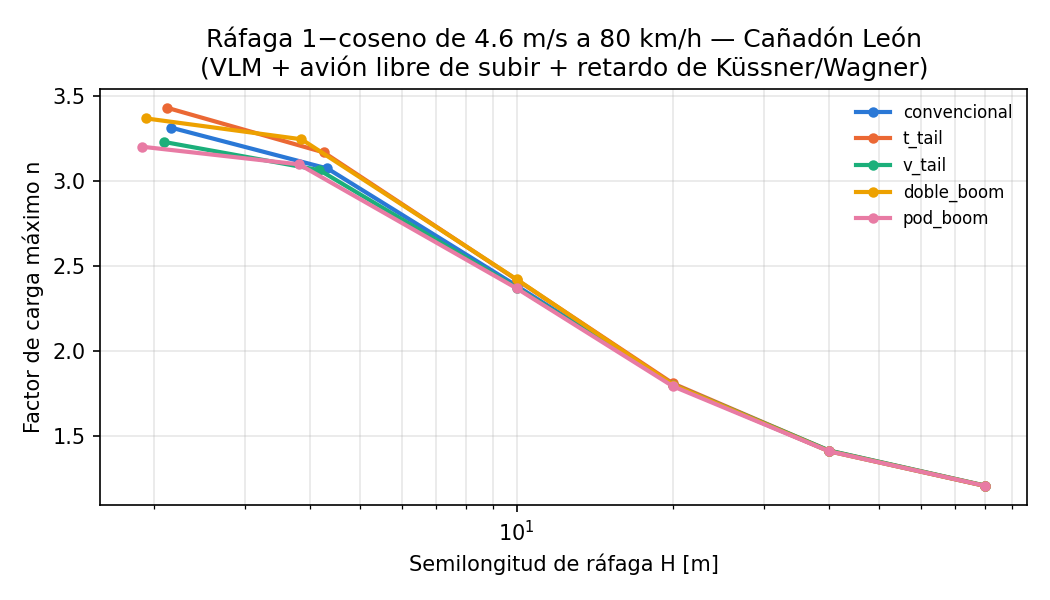
\includegraphics[width=0.8\textwidth]{ganadores_rafaga_barrido_H.png}
\caption{Factor de carga máximo en función de la semilongitud de la ráfaga.
Las ráfagas cortas (del orden de 6--12 cuerdas) son las críticas; las largas
casi no cargan porque el avión sube con ellas.}
\label{fig:barridoH}
\end{figure}

\begin{figure}[H]
\centering
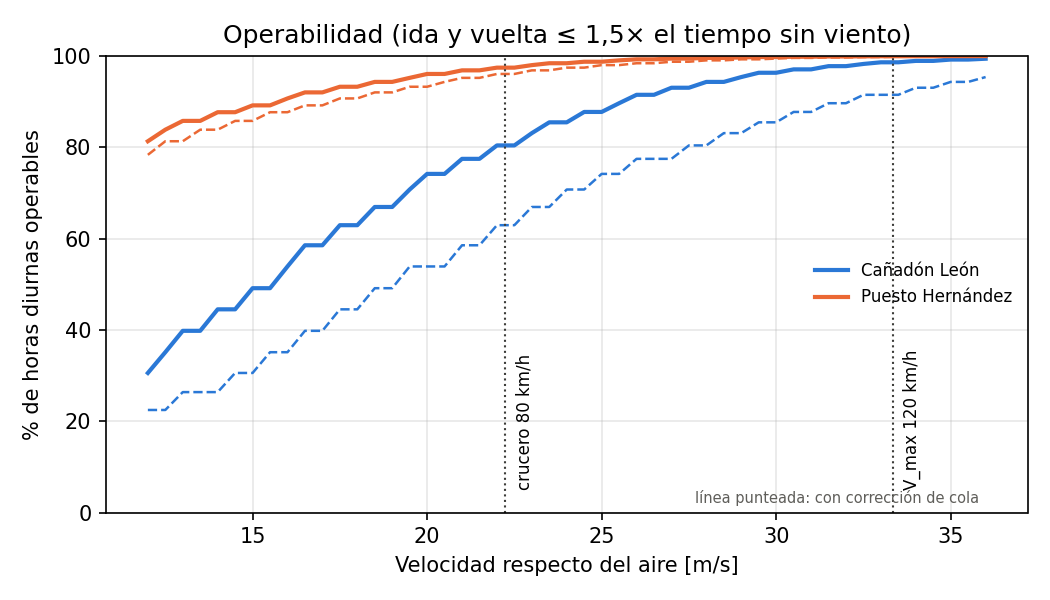
\includegraphics[width=0.8\textwidth]{ganadores_operabilidad_vs_velocidad.png}
\caption{Operabilidad en función de la velocidad respecto del aire, con el
crucero de diseño y la velocidad máxima de la misión actual.}
\label{fig:op-ganadores}
\end{figure}

Conclusiones:
\begin{itemize}
  \item \textbf{Ningún ganador entra en pérdida} con la ráfaga de diseño en
  crucero; el margen va del 18\% (motovelero, Puesto Hernández) al 41\%
  (convencional, Cañadón León).
  \item \textbf{La carga de ráfaga supera levemente el factor de carga límite
  de la estructura.} El optimizador dimensiona con $n_{lim}=3.0$
  ($n_{ult}=4.5$). La ráfaga de diseño a 80~km/h da $n\approx3.1$--$3.4$, y la
  ráfaga de operación a 120~km/h, valores similares. Con la ráfaga de diseño
  a 120~km/h se llega a $n\approx4.2$--$4.6$, en el borde de la carga última.
  Hay dos formas de resolverlo, y la elección es una decisión de diseño:
  subir $n_{lim}$, o adoptar, como CS-23, una ráfaga menor a la velocidad
  máxima (la norma exige la mitad a $V_D$) junto con una limitación operativa
  de velocidad en aire turbulento.
  \item El momento flector en la raíz con ráfaga es entre 3 y 5 veces el de
  vuelo a 1~g. La relación es mayor en las configuraciones cuyo momento a
  1~g es más bajo (cola en T, doble botalón: 19--20~N\,m frente a 26~N\,m
  del convencional), mientras que el momento máximo con ráfaga es parecido en
  todas (70--90~N\,m).
\end{itemize}

Los valores completos por topología y sitio están en la carpeta
\texttt{codigo\_viento/resultados/}, archivos
\texttt{evaluacion\_ganadores\_viento.csv} y
\texttt{rafaga\_vlm\_barrido\_H.csv}.

% ======================================================
\section{Limitaciones}
\label{sec:limitaciones}
% ======================================================

\begin{itemize}
  \item ERA5 representa el promedio de una celda de $\sim$25~km: no
  resuelve efectos locales (bardas, cañadones, estelas de aerogeneradores) ni
  turbulencia de pequeña escala, que por eso se toma de normas.
  \item Diez años alcanzan para la climatología, pero son pocos para
  estimar extremos de período de retorno largo.
  \item Los factores de corrección de cola se derivan de estaciones a 85 y
  180~km de las zonas; son estimaciones, no correcciones exactas.
  \item La operabilidad supone el peor caso (viento alineado con la ruta) y
  potencia constante; con viento cruzado el resultado es más favorable.
  \item La respuesta dinámica a ráfagas usa un solo grado de libertad
  (ascenso) y las funciones de Küssner y Wagner de un perfil 2D; no incluye
  cabeceo, alivio inercial del peso del ala ni flexibilidad. Un VLM no
  estacionario (UVLM) con dinámica de vuelo completa sería el paso siguiente.
\end{itemize}

% ======================================================
\section{Próximos pasos}
\label{sec:proximos}
% ======================================================

\begin{enumerate}
  \item Decidir con el grupo la \textbf{ráfaga de diseño} (propuesta:
  4.6~m/s) y el \textbf{factor de carga límite} de la estructura, dado que
  hoy se usa $n_{lim}=3.0$ y la ráfaga de diseño da $n\approx3.1$--$3.4$
  (Sección~\ref{sec:codigo}).
  \item Decidir, junto con quien mantiene el optimizador, si se incorporan
  al puntaje la densidad y la ráfaga del sitio (las funciones de
  \texttt{mision\_viento} están pensadas para eso) en lugar de 1.225~kg/m$^3$
  y 3~m/s.
  \item Pasar el momento flector en la raíz con ráfaga al dimensionamiento
  del larguero.
  \item Extender la respuesta dinámica a dos grados de libertad (ascenso y
  cabeceo) y analizar despegue/aterrizaje con cortante vertical.
  \item Solicitar a Quintana / YPF datos de estaciones meteorológicas propias
  en los yacimientos para reemplazar o validar los factores de corrección.
\end{enumerate}

% ======================================================
\section*{Referencias}
% ======================================================

{\small\sloppy
\begin{itemize}[leftmargin=*]
  \item Hersbach, H. et al. (2020). The ERA5 global reanalysis.
  \textit{Q. J. R. Meteorol. Soc.}, 146, 1999--2049.
  \item Open-Meteo, Historical Weather API:
  \url{https://open-meteo.com/en/docs/historical-weather-api}
  \item NOAA NCEI, Global Hourly (ISD), estaciones 87860099999 y 87715099999:
  \url{https://www.ncei.noaa.gov/access/services/data/v1?dataset=global-hourly}
  \item MIL-F-8785C y MIL-HDBK-1797, modelo de turbulencia de Dryden
  (resumen en MathWorks, \textit{Dryden Wind Turbulence Model}):
  \url{https://www.mathworks.com/help/aeroblks/drydenwindturbulencemodelcontinuous.html}
  \item 14 CFR \S23.333 (envolvente de ráfaga) y \S23.341 (factores de carga
  por ráfaga):
  \url{https://www.govinfo.gov/content/pkg/CFR-2011-title14-vol1/pdf/CFR-2011-title14-vol1-sec23-333.pdf}
  \item Pérez, C. L. (2018). Caracterización petrofísica del yacimiento
  Cañadón León. IAPG, 10º Congreso de Exploración y Desarrollo de
  Hidrocarburos.
  \item Groba, C., Marteau, M., Romera, W. Proyecto de perforación de pozos
  interdistanciados en la Formación Rayoso, yacimiento Puesto Hernández. IAPG.
\end{itemize}
}

\end{document}
